
% %map showing core locations
% \begin{figure}
% \centering
% 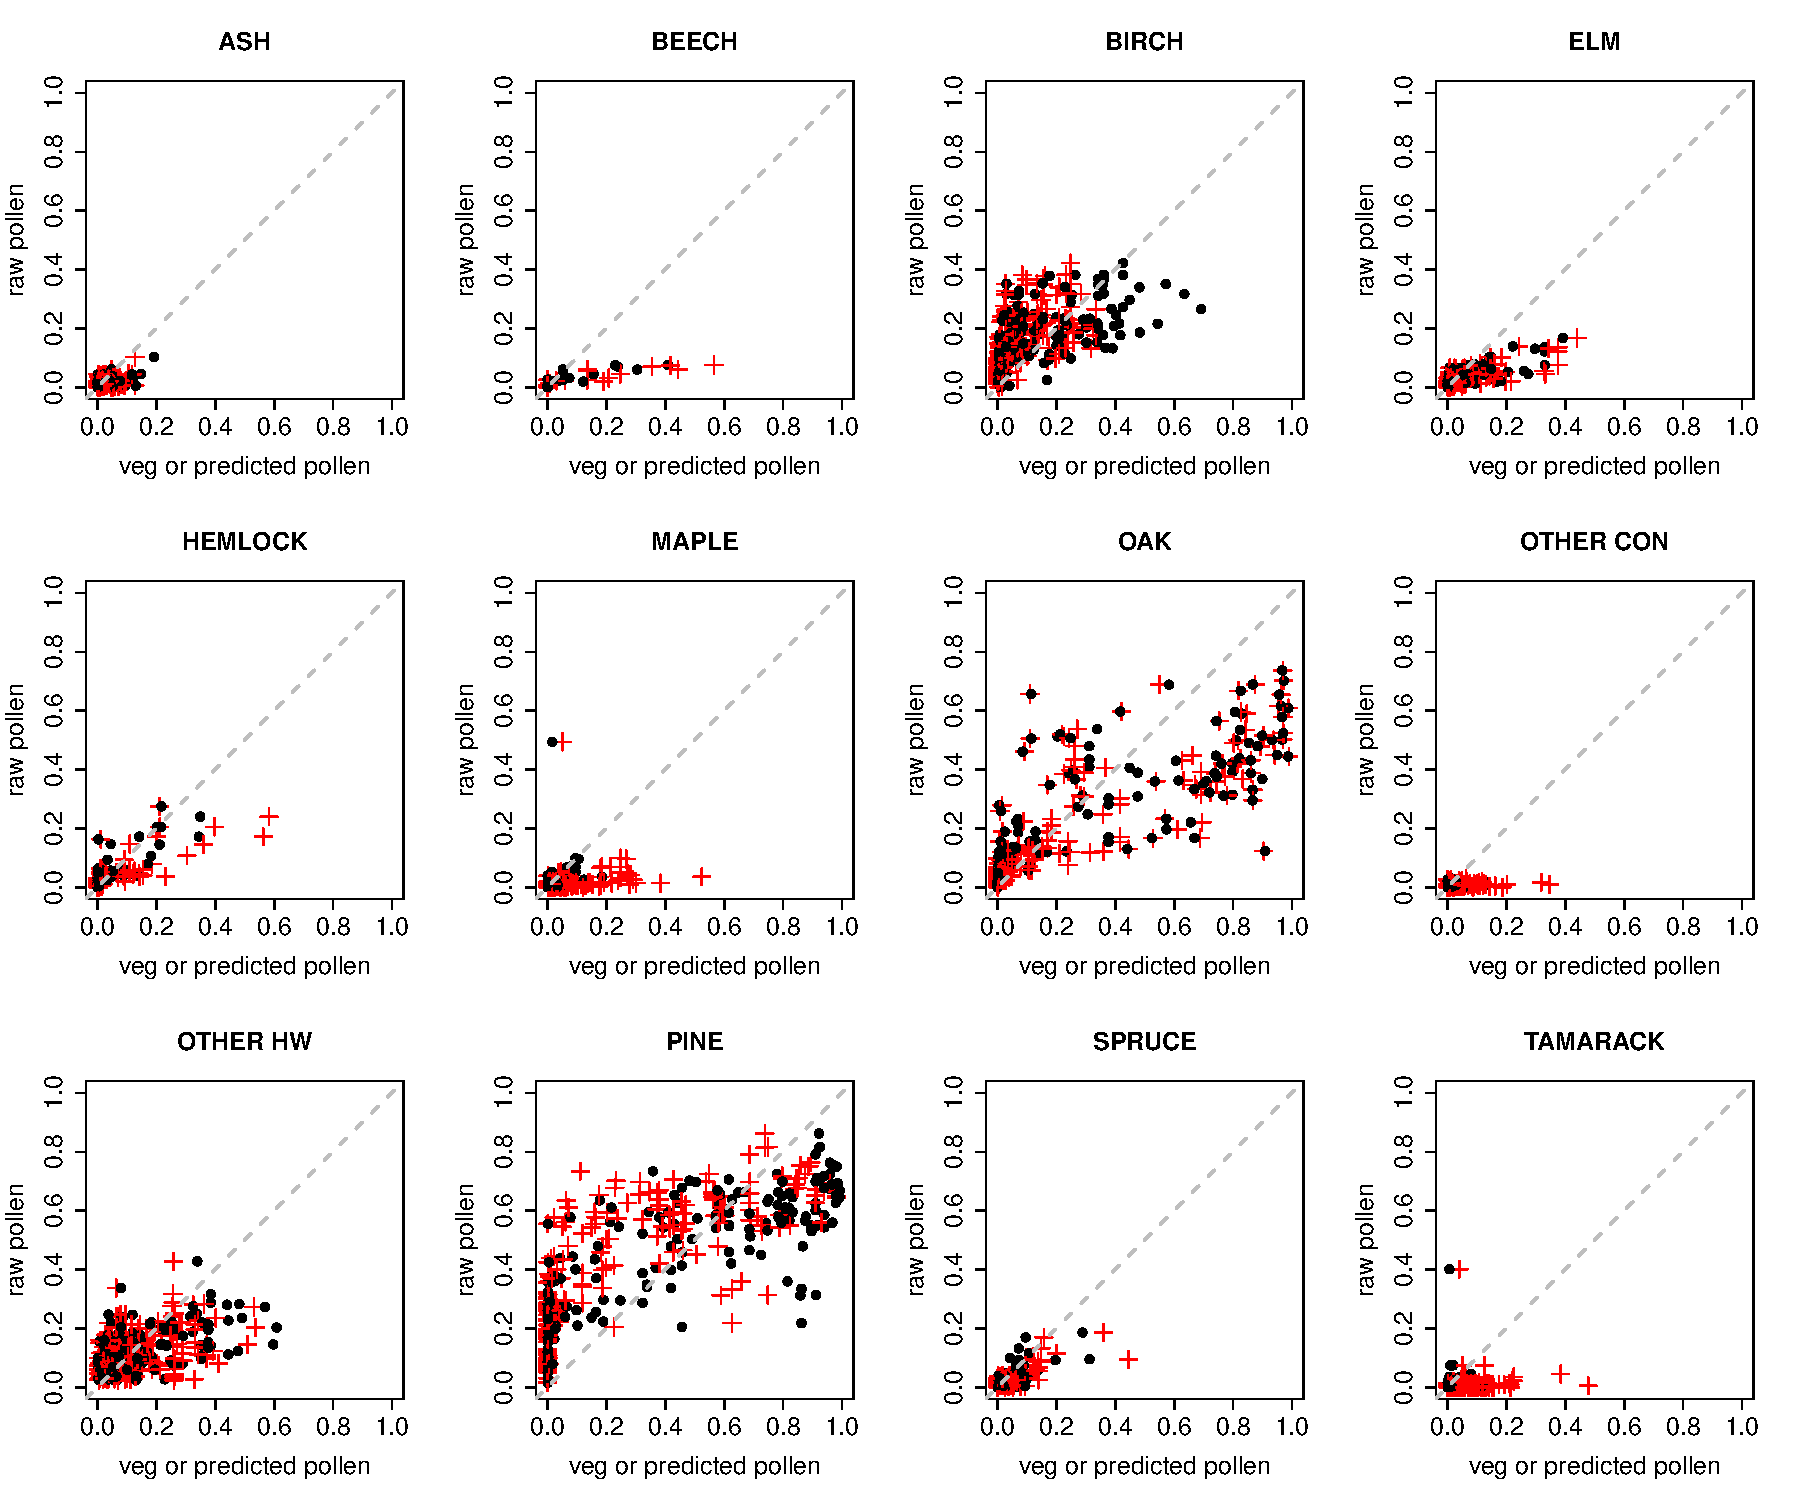
\includegraphics[width=7in]{figures/pollen_focal_scaled.pdf}
% \caption{}
% \label{fig:focal_scaled}
% \end{figure}

%PLS and pollen pie maps
\begin{figure}
\centering
\begin{tabular}{c}
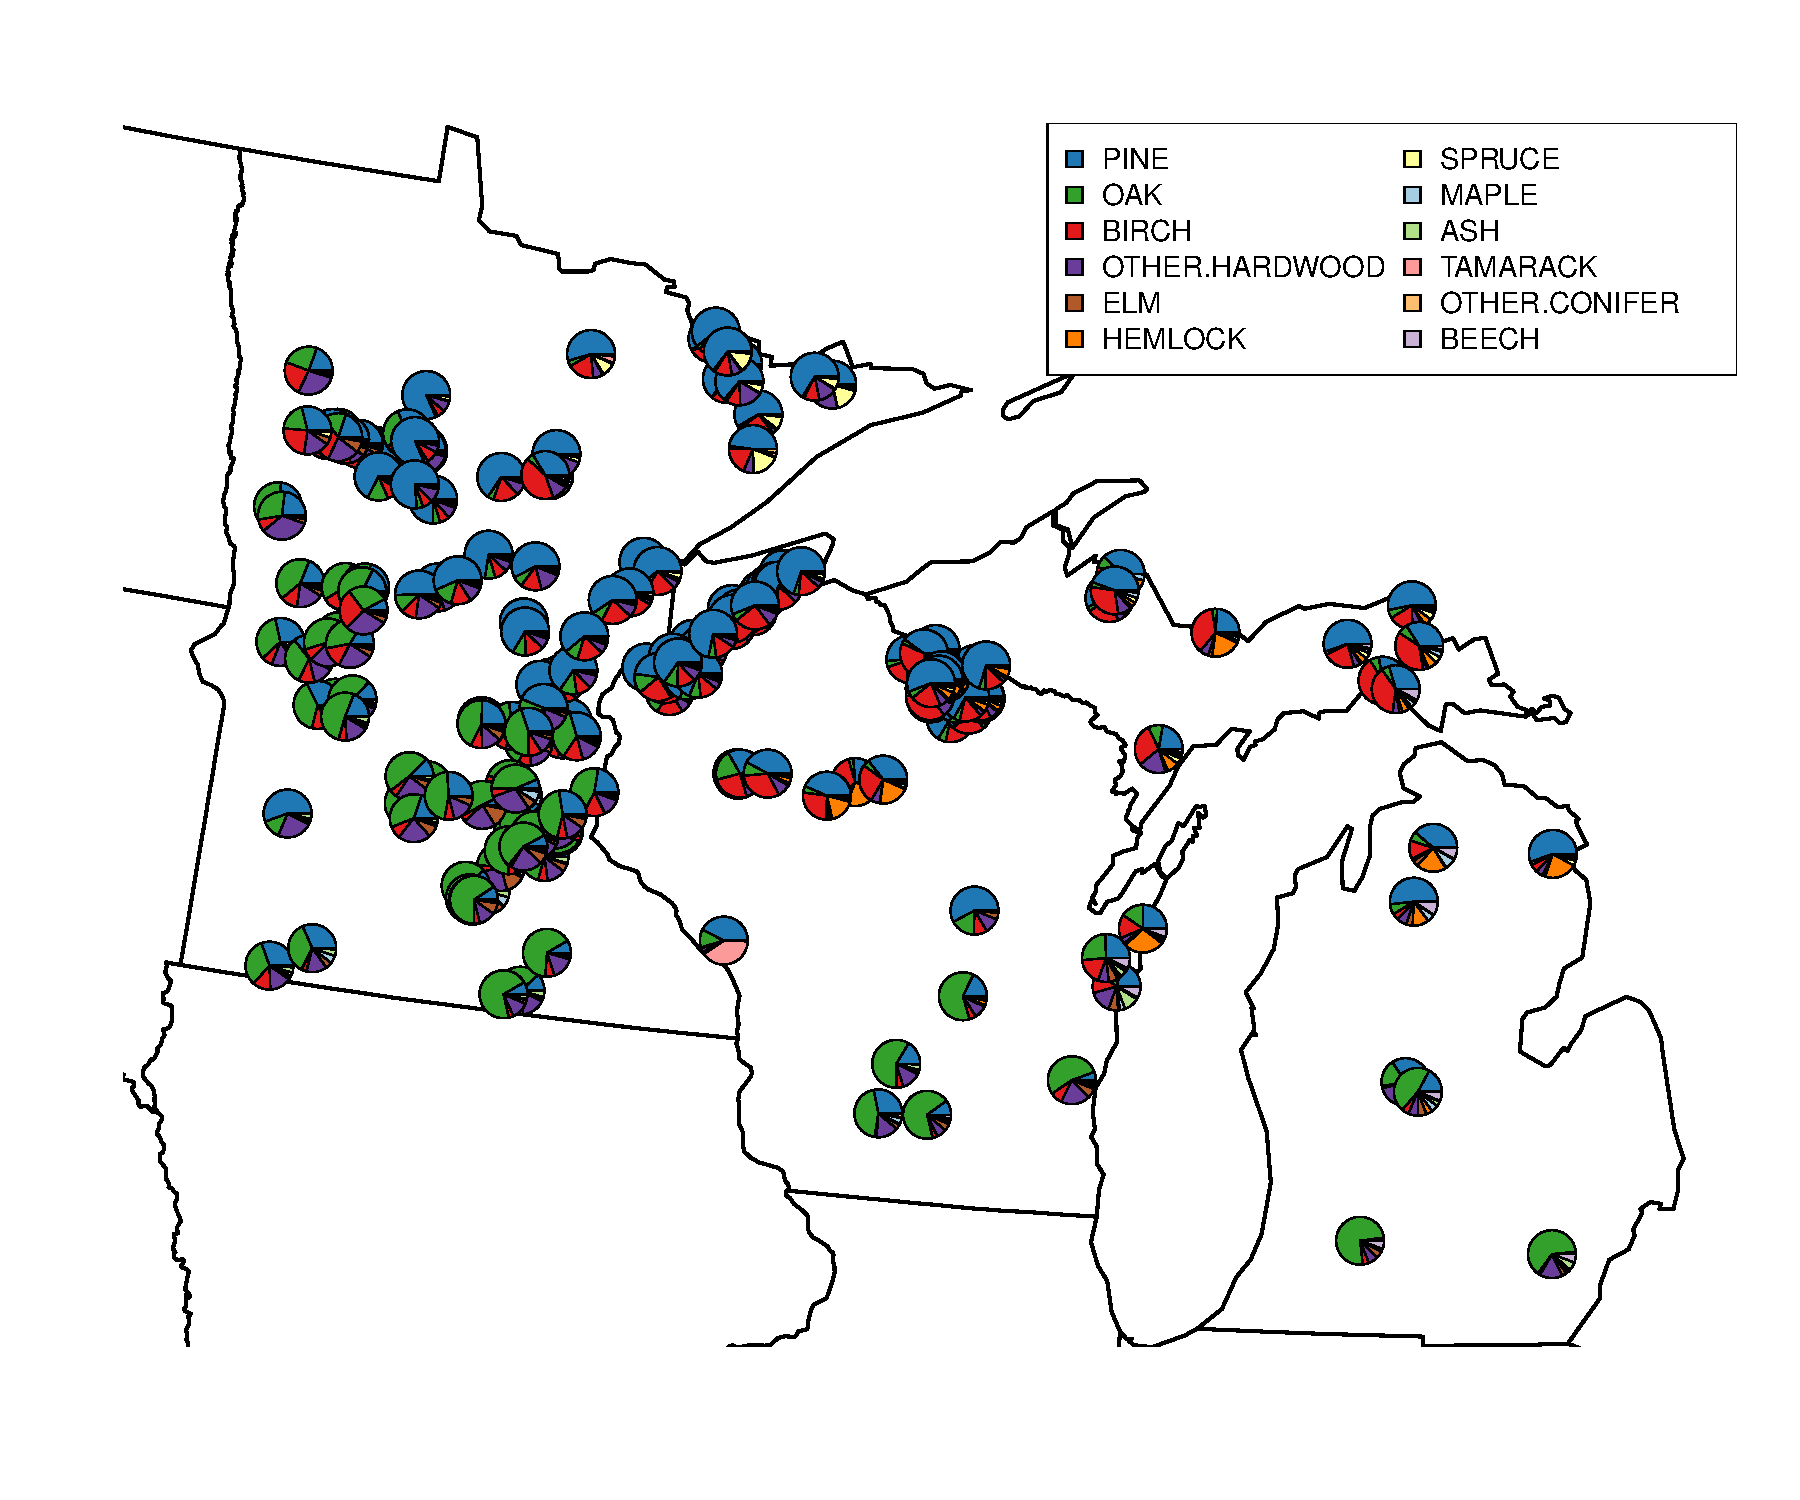
\includegraphics[width=5in]{figures/pie_plot_pollen_ALL_v0_3.pdf} \\
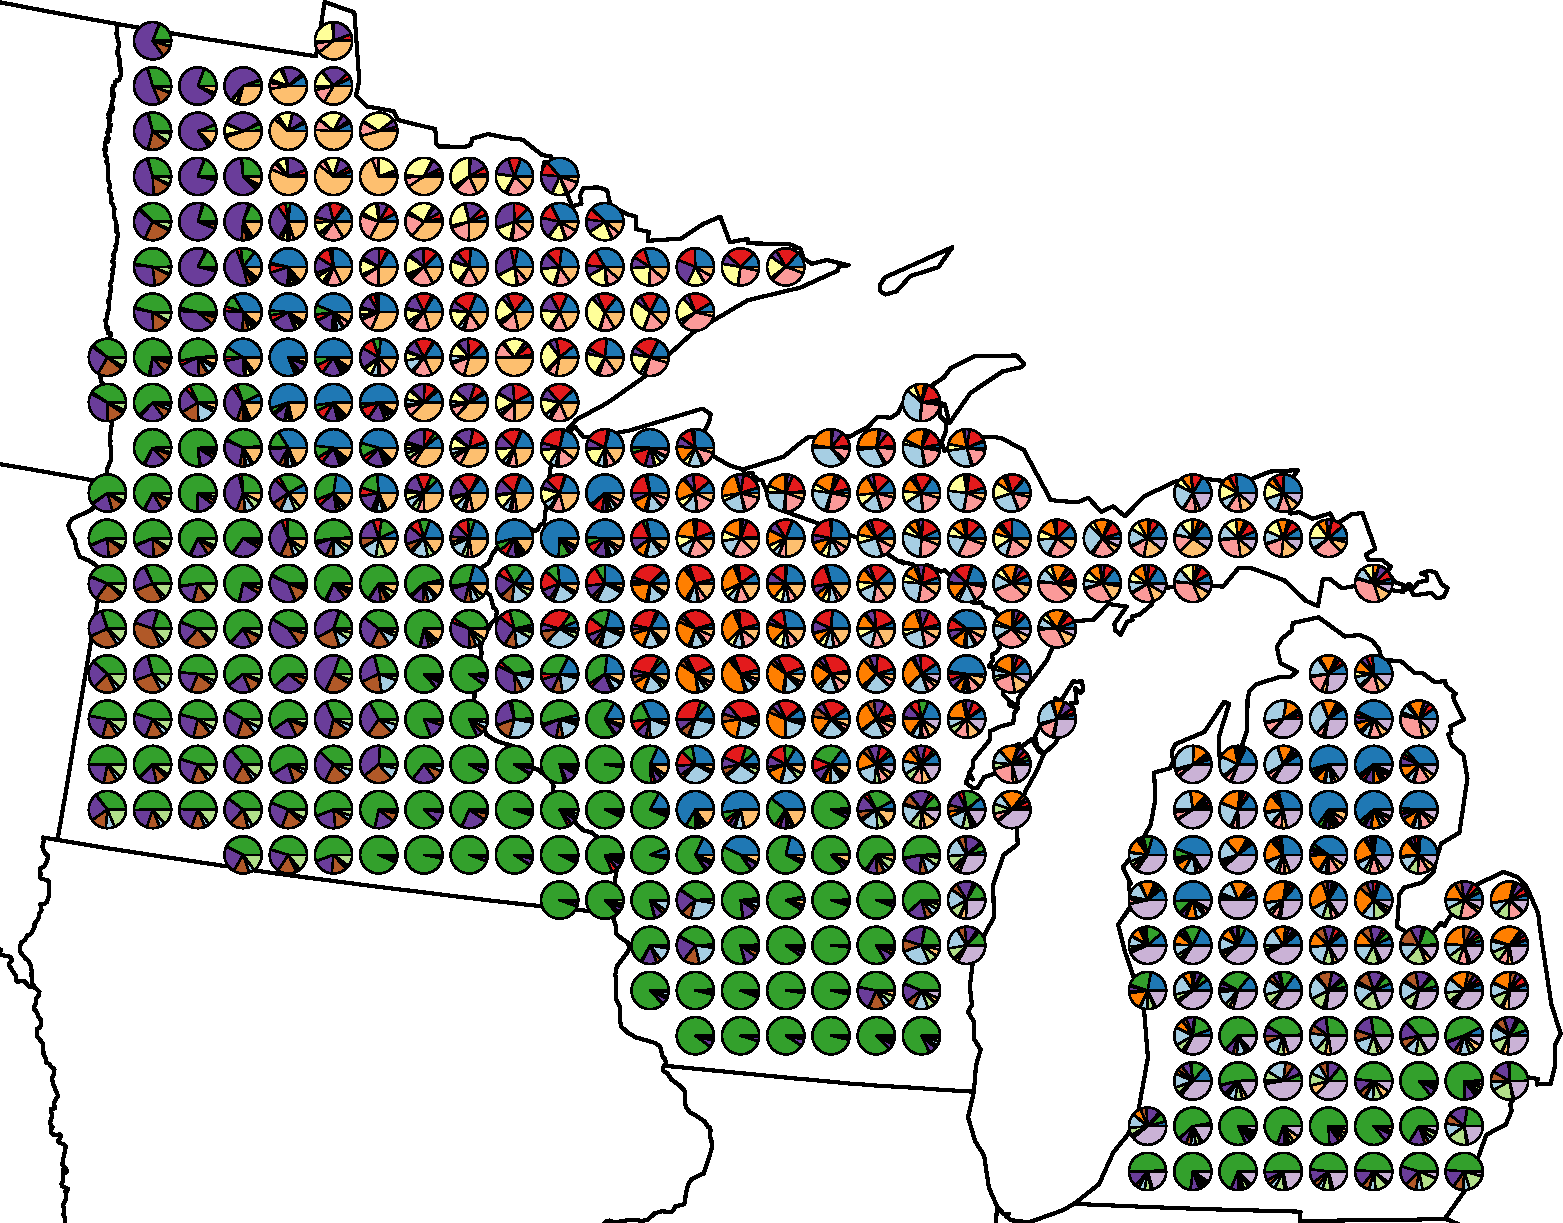
\includegraphics[width=5in]{figures/pie_plot_pls_ALL_v0_3.pdf}
\end{tabular}
\caption{Pie maps depicting the relative composition of pollen (top)
  and PLS vegetation (bottom) from the data. Note that the PLS data
  has been aggregated to a coarser resolution for illustrative
  purposes.}
\label{fig:pie}
\end{figure}

%trace plots
\begin{figure}
\centering
\begin{tabular}{ccc}
%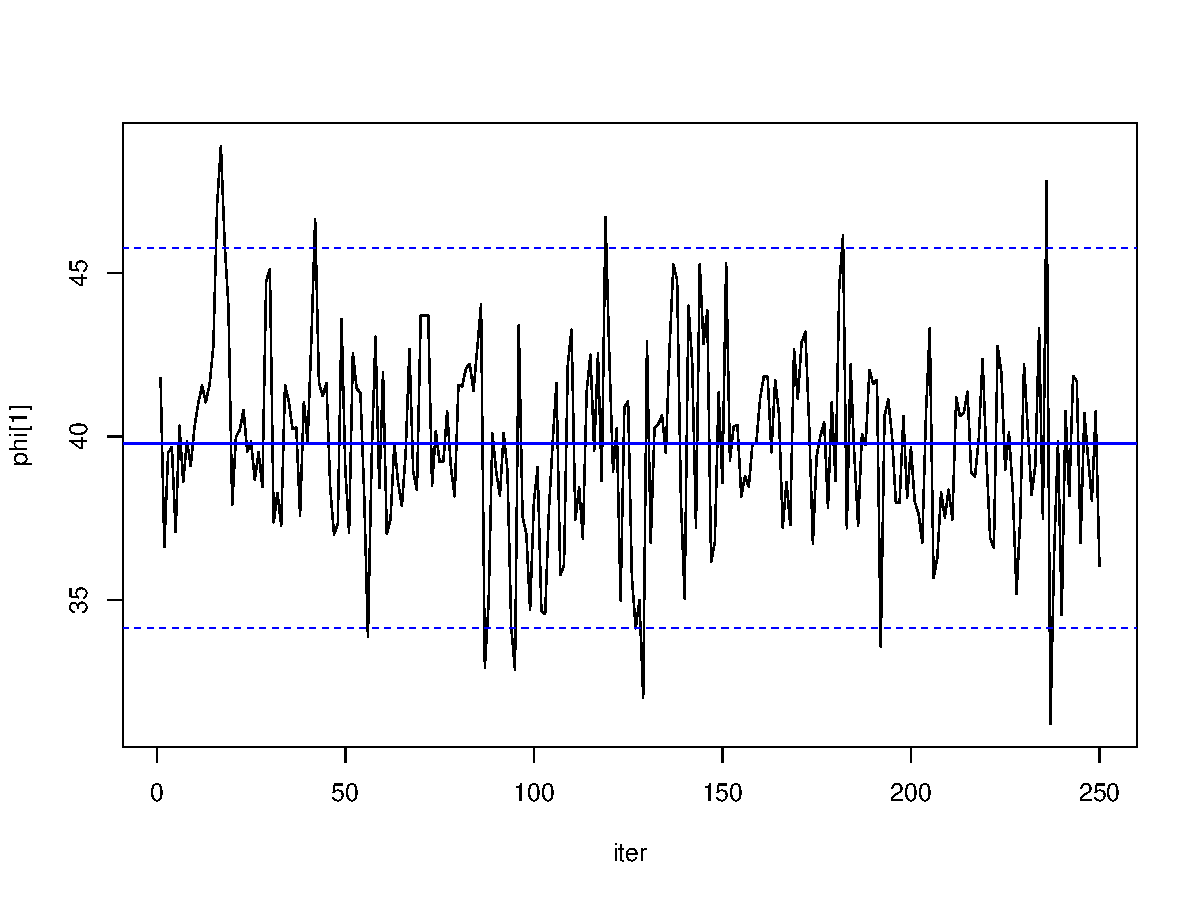
\includegraphics[width=5in]{figures/cal_trace.pdf}
%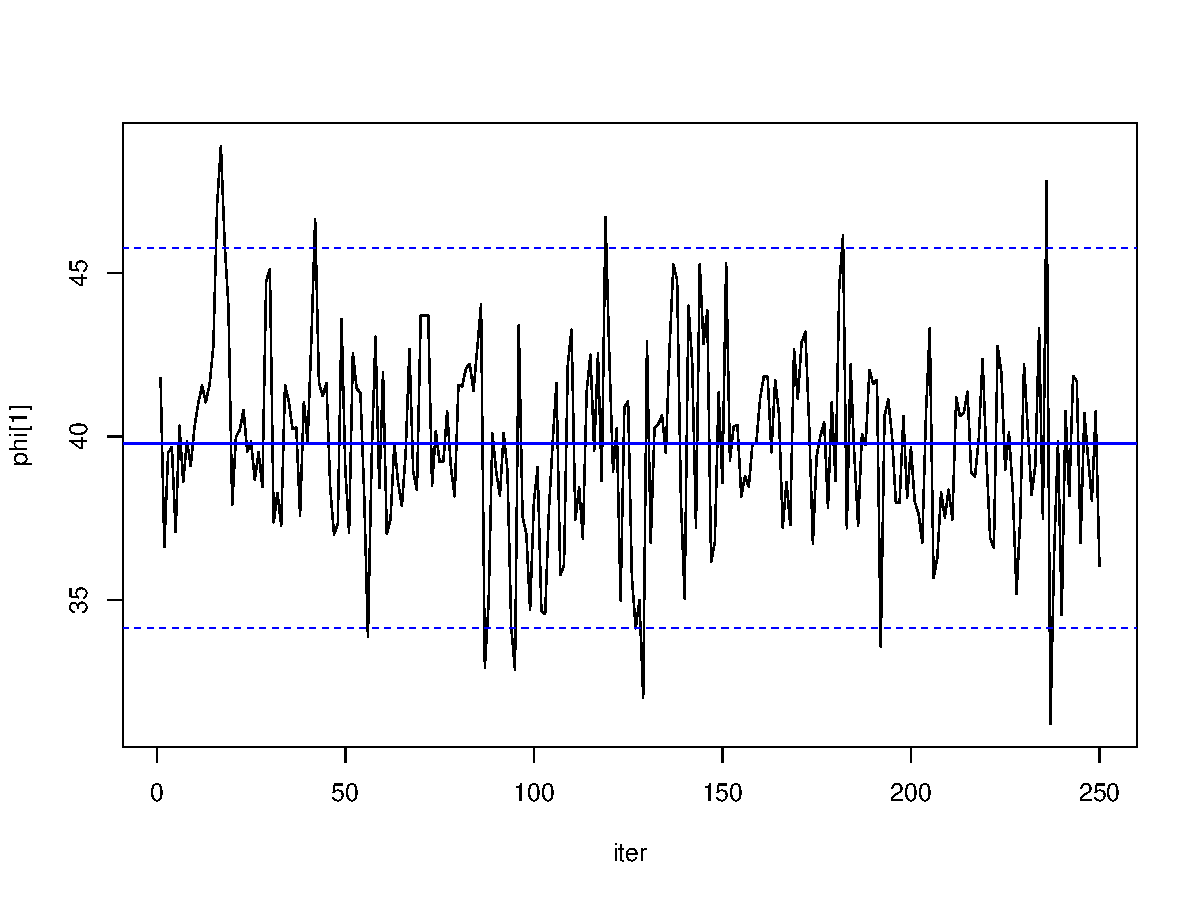
\includepdf[nup=2x3]{figures/cal_trace.pdf}
  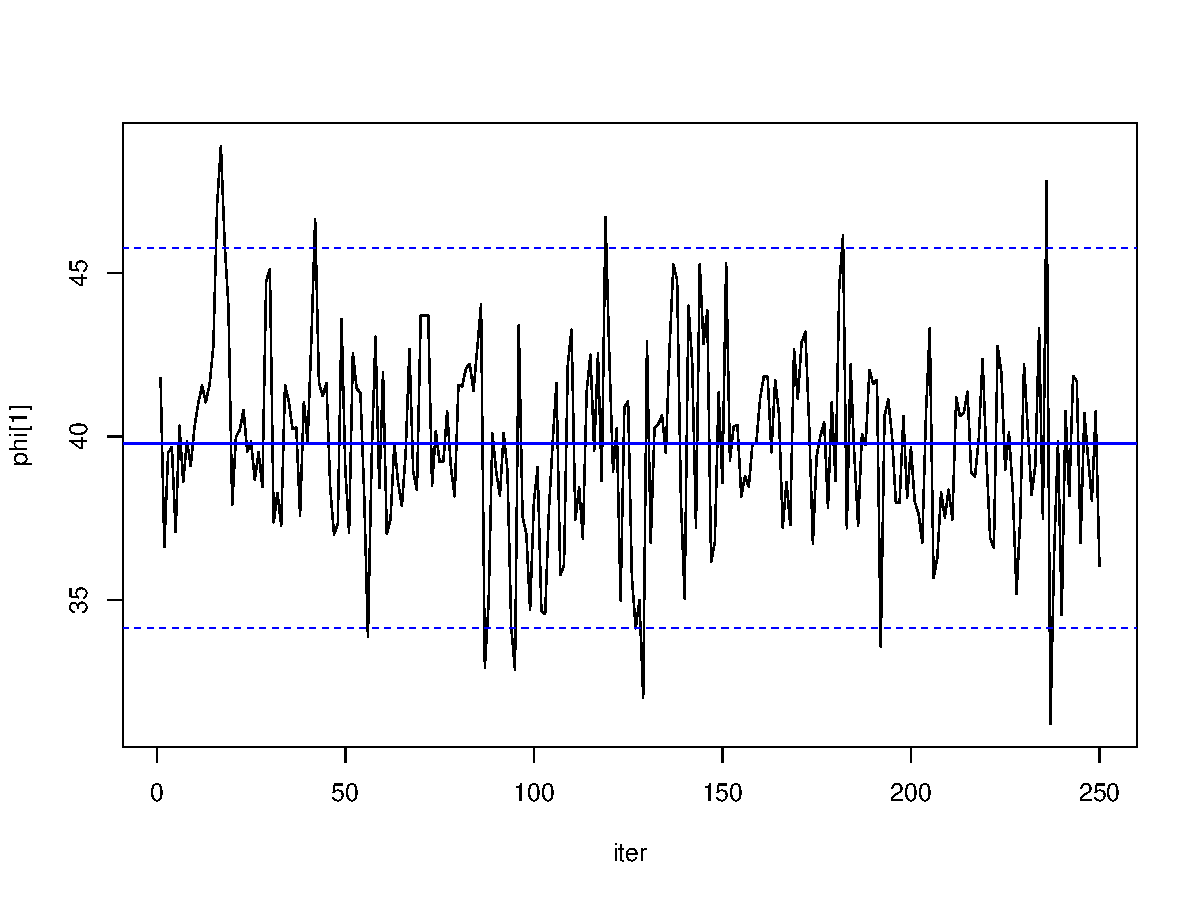
\includegraphics[page=1,width=0.3\textwidth]{figures/cal_trace.pdf} &
  \includegraphics[page=2,width=0.3\textwidth]{figures/cal_trace.pdf} &
  \includegraphics[page=3,width=0.3\textwidth]{figures/cal_trace.pdf} \\
  \includegraphics[page=4,width=0.3\textwidth]{figures/cal_trace.pdf} &
  \includegraphics[page=5,width=0.3\textwidth]{figures/cal_trace.pdf} &
  \includegraphics[page=6,width=0.3\textwidth]{figures/cal_trace.pdf} \\
  \includegraphics[page=7,width=0.3\textwidth]{figures/cal_trace.pdf} &
  \includegraphics[page=8,width=0.3\textwidth]{figures/cal_trace.pdf} &
  \includegraphics[page=9,width=0.3\textwidth]{figures/cal_trace.pdf} \\
  \includegraphics[page=10,width=0.3\textwidth]{figures/cal_trace.pdf} &
  \includegraphics[page=11,width=0.3\textwidth]{figures/cal_trace.pdf} &
  \includegraphics[page=12,width=0.3\textwidth]{figures/cal_trace.pdf} \\
  \includegraphics[page=13,width=0.3\textwidth]{figures/cal_trace.pdf} &
  \includegraphics[page=14,width=0.3\textwidth]{figures/cal_trace.pdf} &
  \includegraphics[page=15,width=0.3\textwidth]{figures/cal_trace.pdf} 
\end{tabular}
\caption{Trace plots for the parameters in the gaussian dispersed
  calibration model, including $\phi_k$ for $k=1, \ldots, W$, $\psi$,
  and $\gamma$, as well as the joint log posterior,
  $\text{lp}$. Posterior estimates for each of the three runs are
  depicted in shades of grey. The 2.5\% and 97.5\% quantiles are
  indicated by the solid lines, while the 50\% quantiles are indicated
  by the hashed lines.}
\label{fig:trace}
\end{figure}

%veg and pollen heat maps: pine
\begin{figure}
\centering
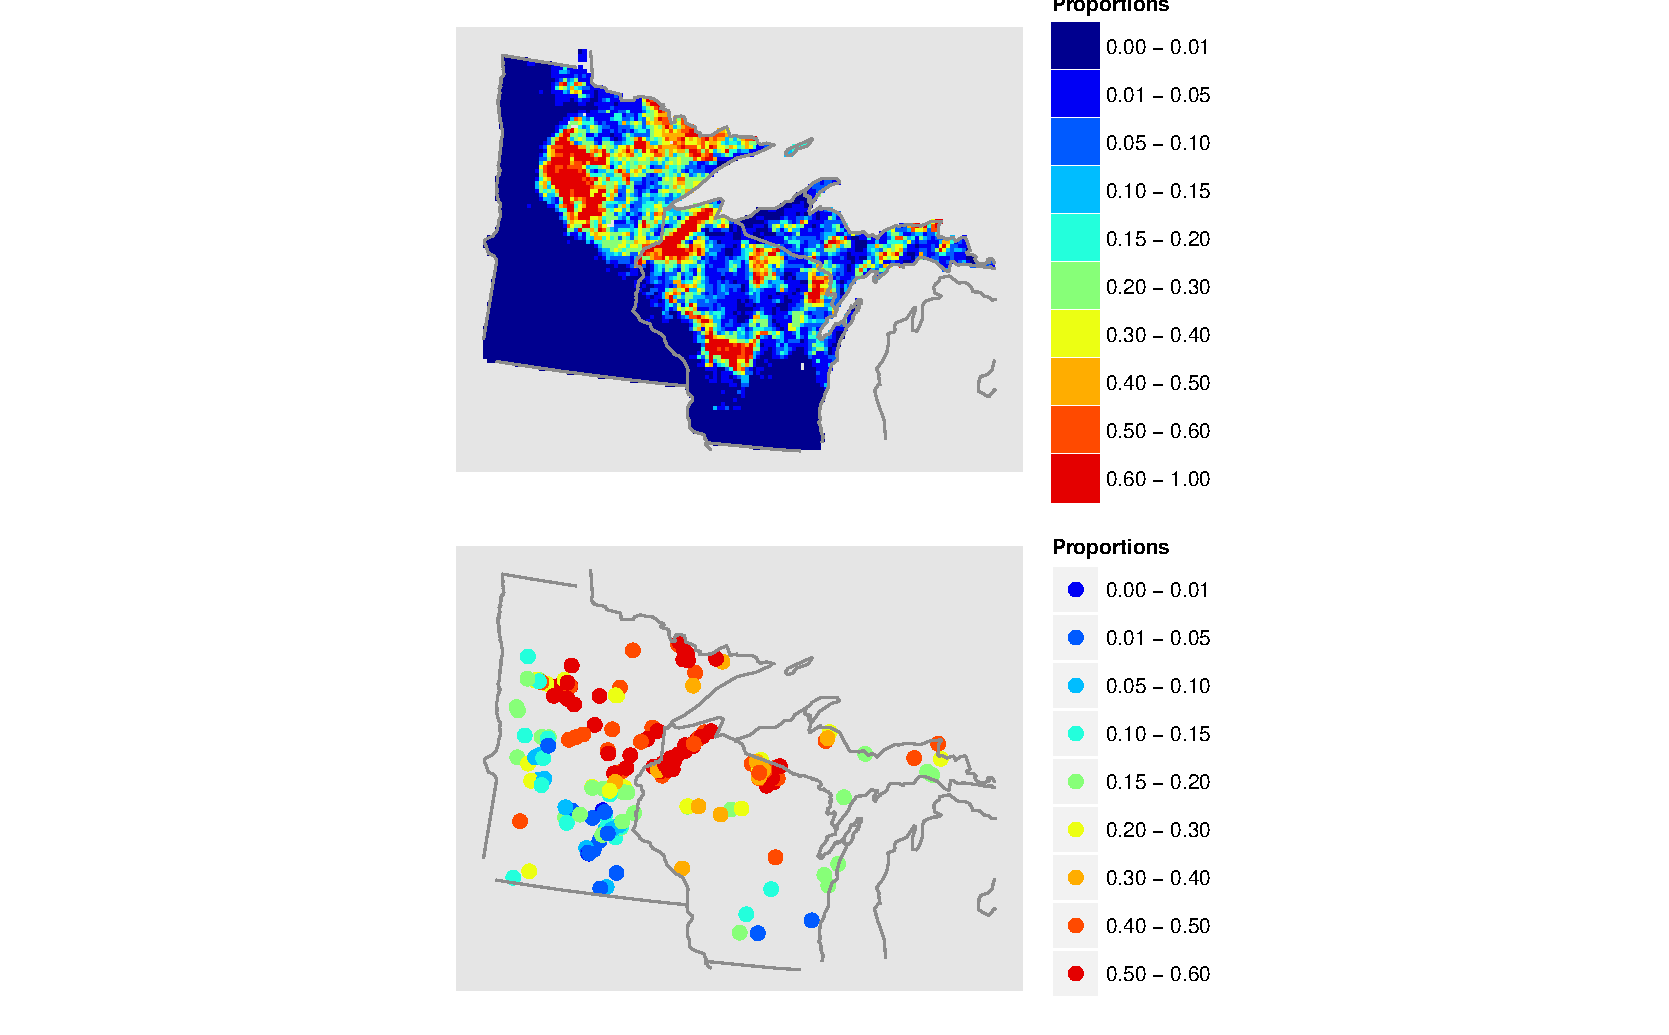
\includegraphics[width=7in]{figures/maps_compare_PINE.pdf}
\caption{Heat maps showing the range limits of Pine in the PLS
  composition data (top) and the pre-settlement calibration sediment
  pollen data (bottom).}
\label{fig:compare_maps_PINE}
\end{figure}

%veg and pollen heat maps: birch
\begin{figure}
\centering
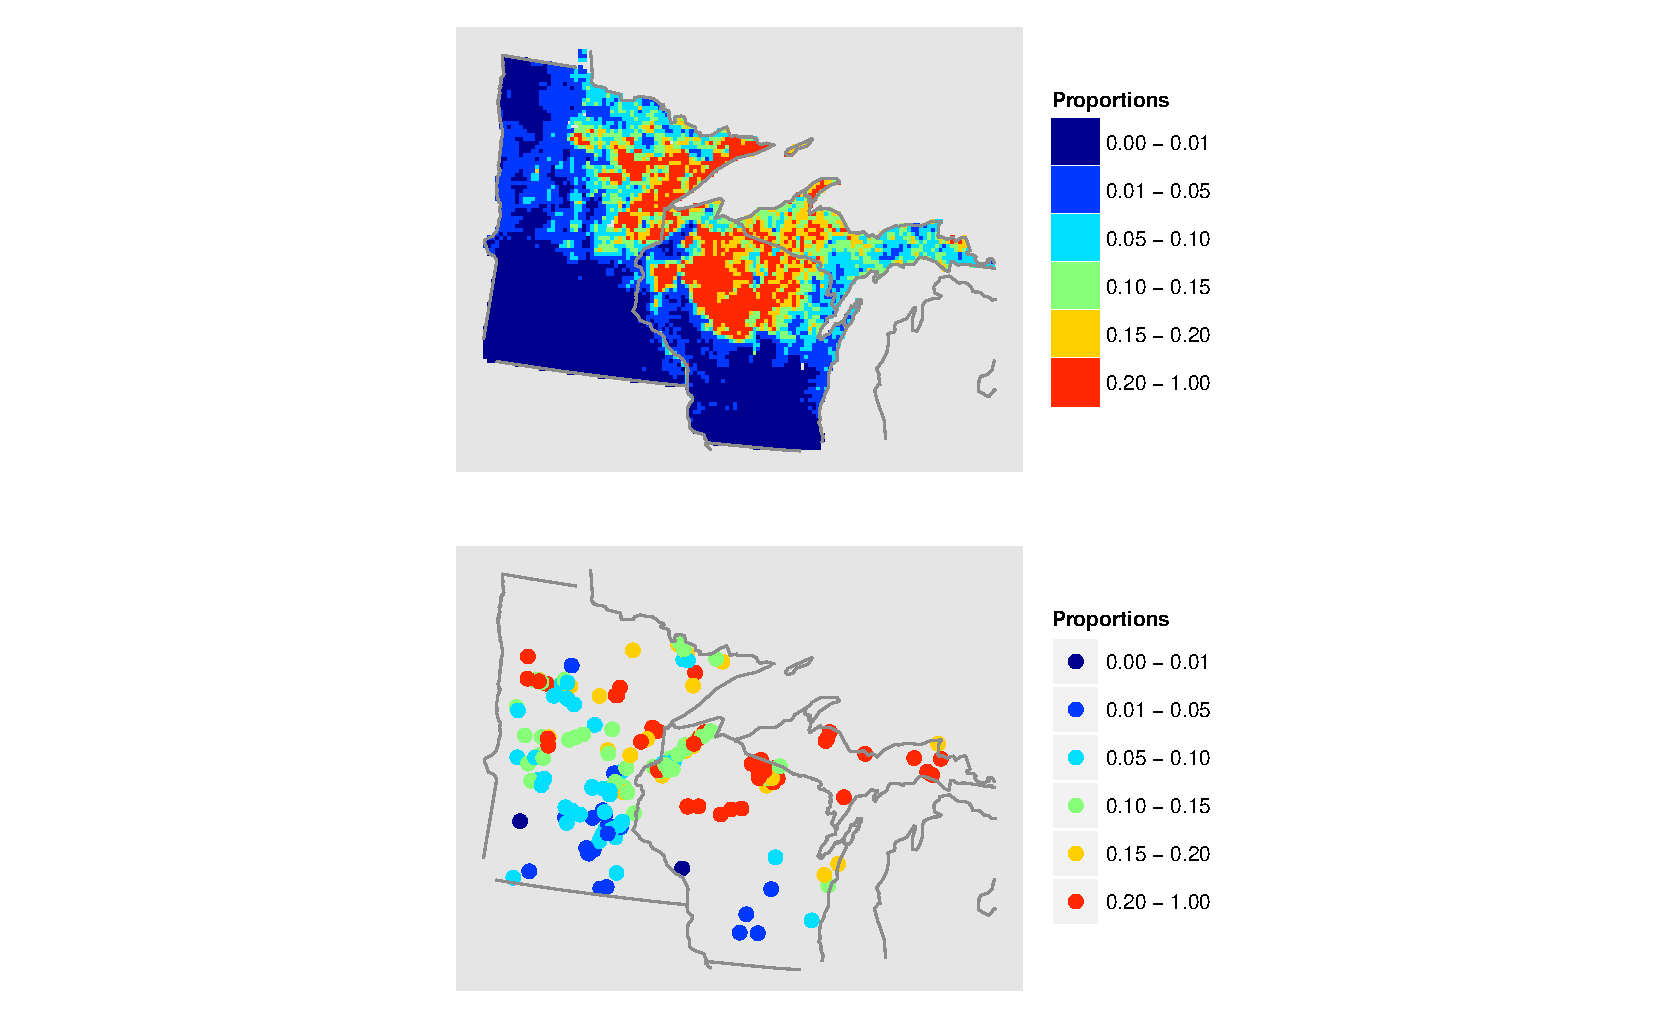
\includegraphics[width=7in]{figures/maps_compare_BIRCH.pdf}
\caption{Heat maps showing the range limits of Birch in the PLS
  composition data (top) and the pre-settlement calibration sediment
  pollen data (bottom)}
\label{fig:compare_maps_BIRCH}
\end{figure}

%pollen raw versus scaled focal
\begin{figure}
\centering
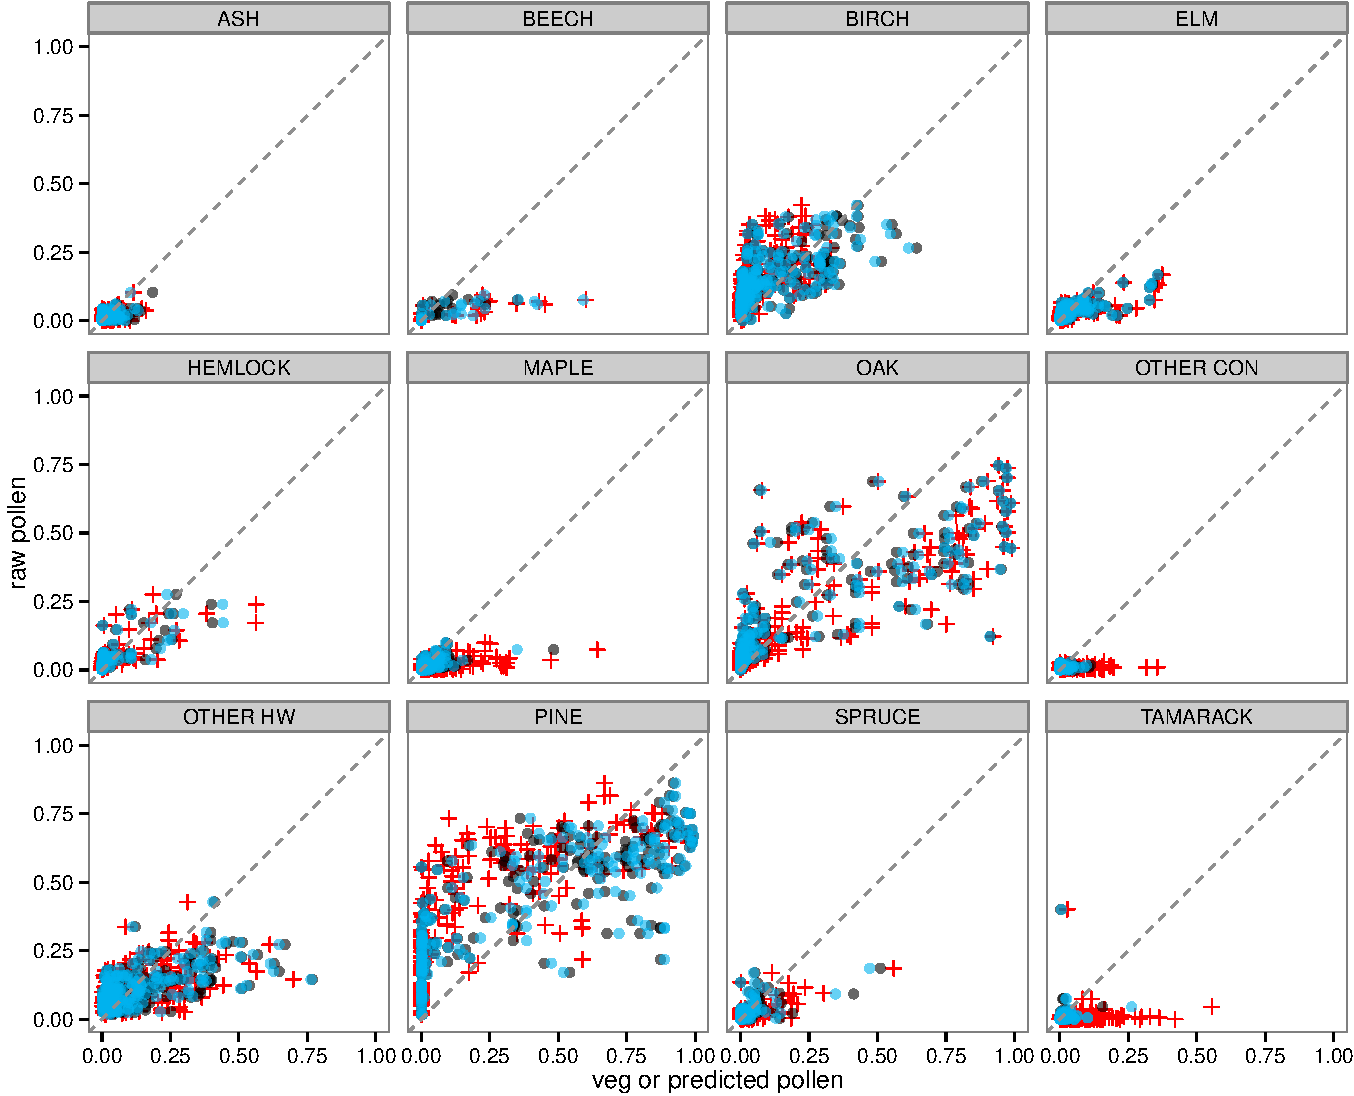
\includegraphics[width=7in]{figures/pollen_phi_scaled_flexible.pdf}
\caption{Pollen proportions plotted against local vegetation proportions (red crosses) or local vegetation proportion scaled by $\bm{\phi}$ for the variable gaussian kernel model (black dots) and the variable power law kernel model (blue dots), by taxon.}
\label{fig:focal_scaled}
\end{figure}

%pollen raw versus predicted
\begin{figure}
\centering
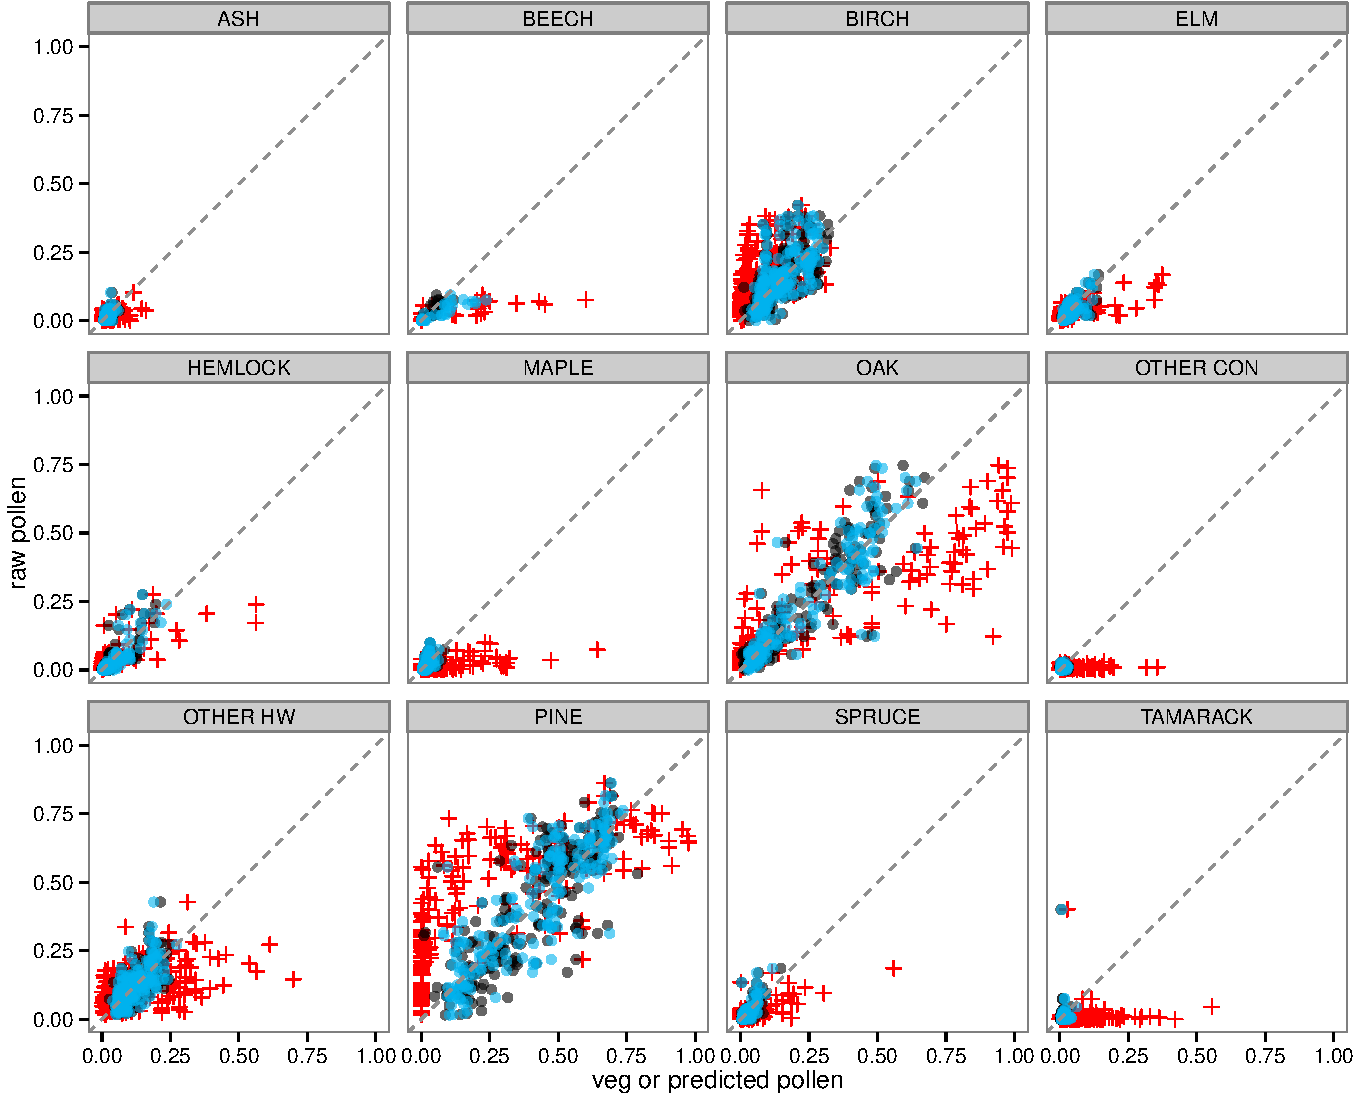
\includegraphics[width=7in]{figures/pollen_preds_flexible.pdf}
\caption{Pollen proportions plotted against local vegetation proportions (red crosses) or model-predicted pollen for the variable gaussian kernel model (black dots) and the variable power law kernel model (blue dots), by taxon.}
\label{fig:preds}
\end{figure}

%phi (differential production)
\begin{figure}
\centering
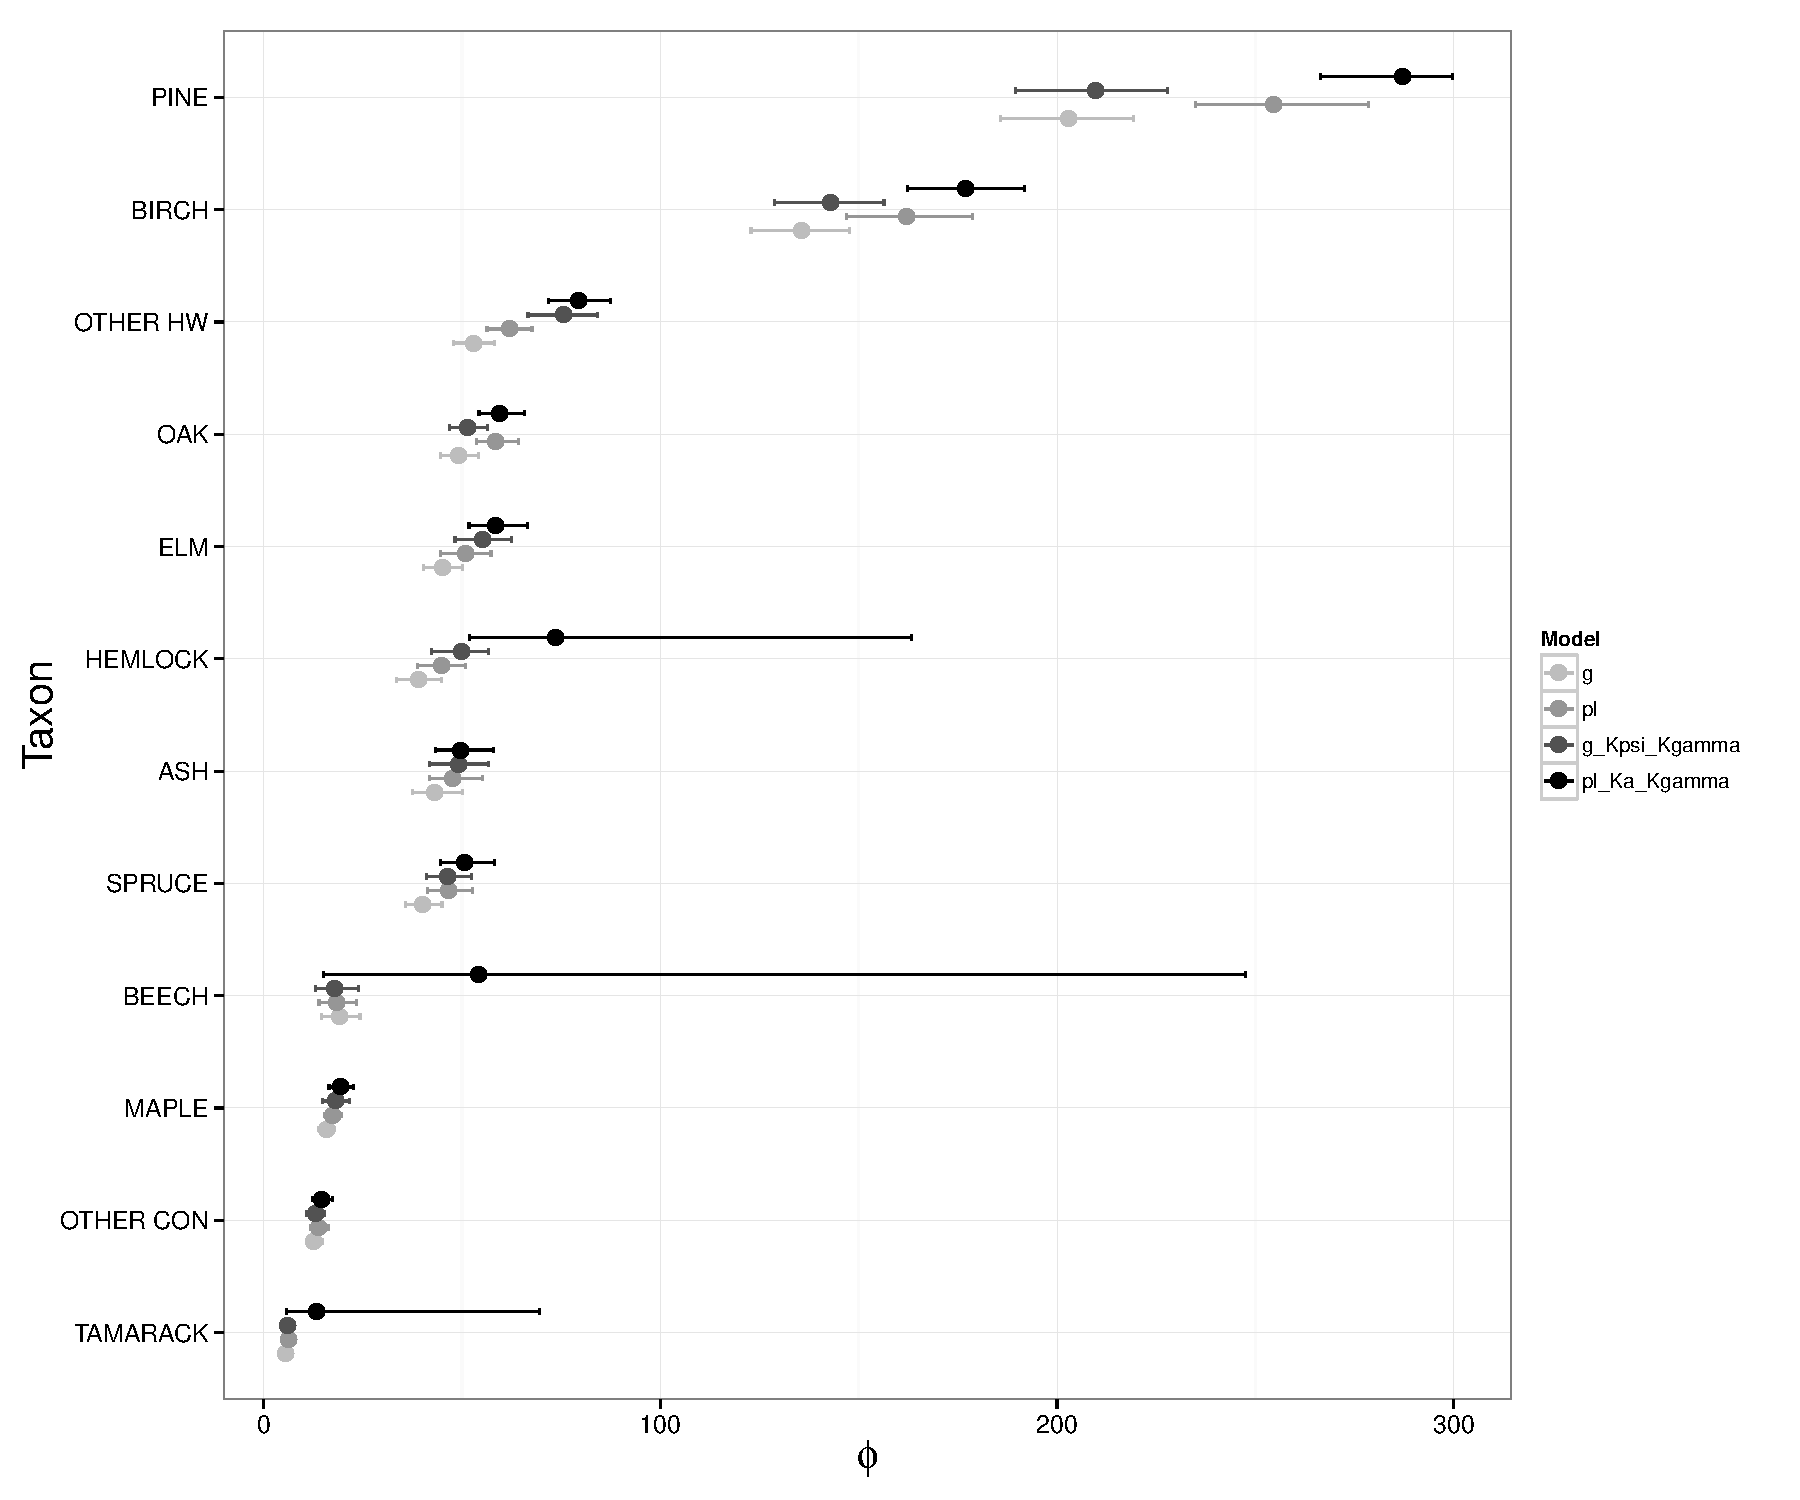
\includegraphics[width=7in]{figures/phi.pdf}
\caption{Mean values and 95\% credible intervals for the estimated values of the differential production parameter $\phi$.}
\label{fig:phi}
\end{figure}

%proportion pollen versus radius
\begin{figure}
\centering
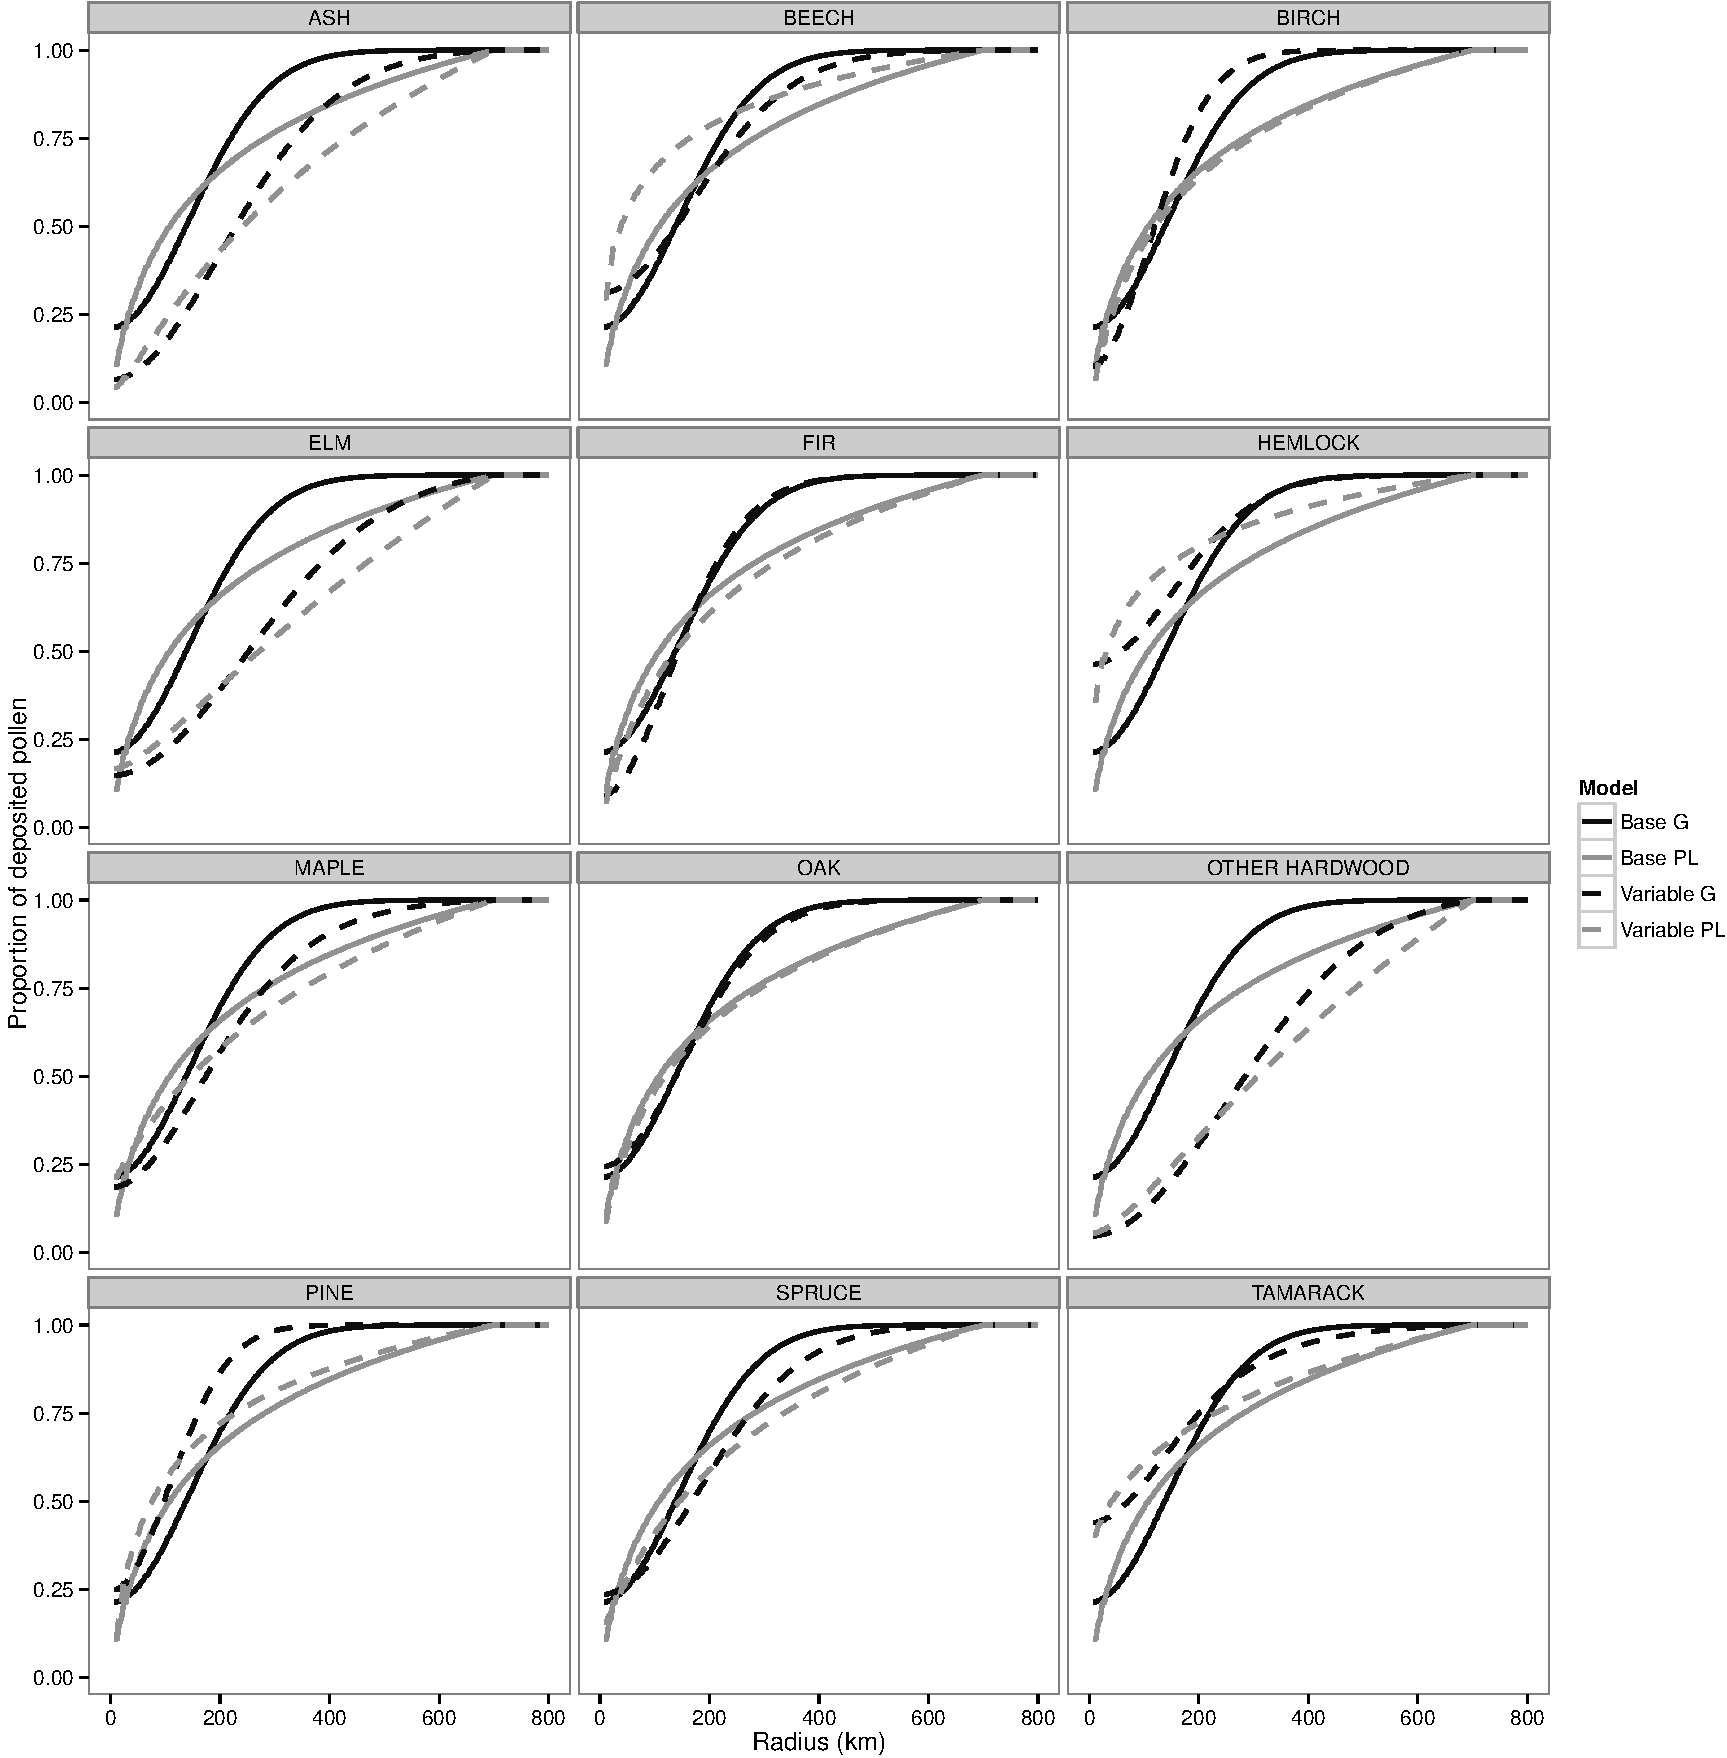
\includegraphics[width=7in]{figures/kernel_discrete_cdfs.pdf}
\caption{For each of the four considered models (gaussian base and
  variable; power law base and variable), the proportion of deposited
  (or accumulated) pollen is plotted as a function of radius for each
  of the modelled taxa.}
\label{fig:dvd}
\end{figure}

% %psi: variable gaussian
% \begin{figure}
% \centering
% 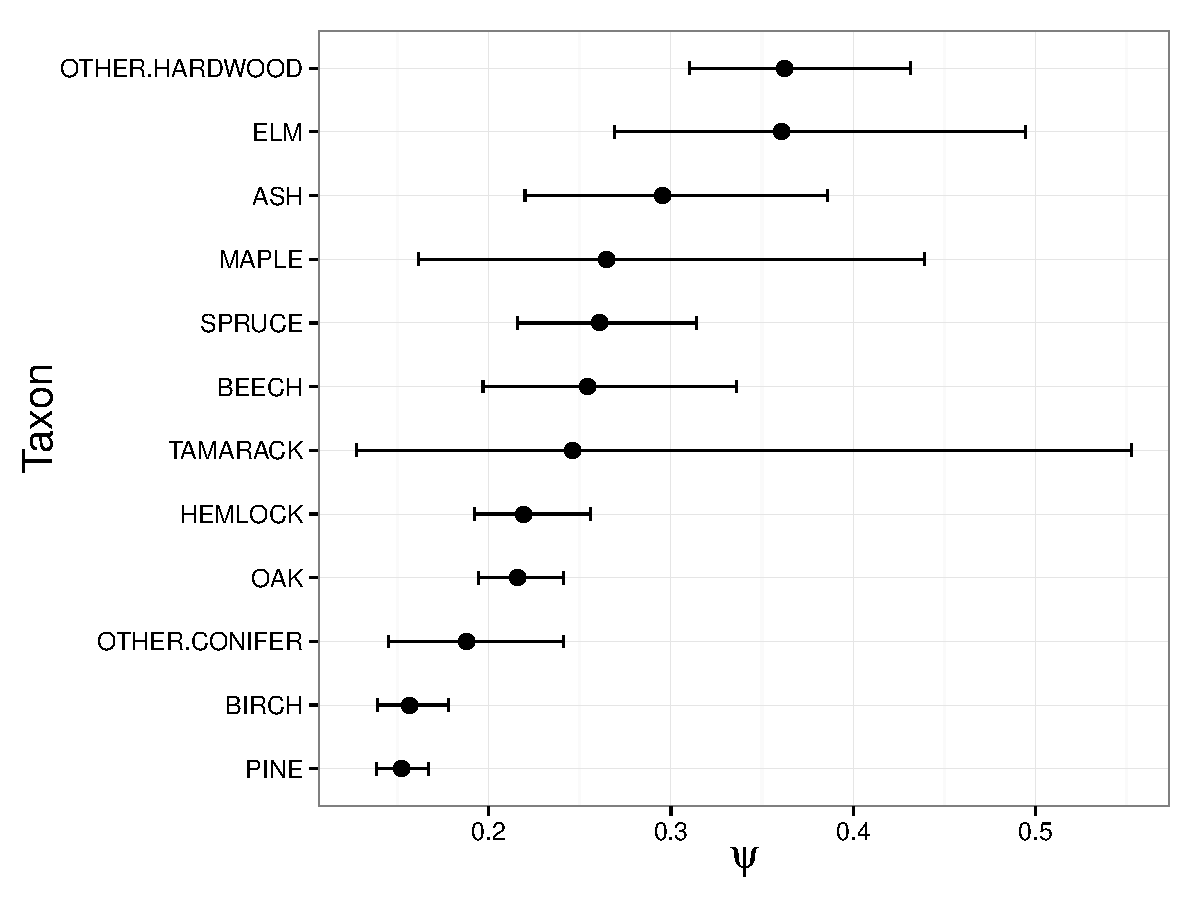
\includegraphics[width=7in]{figures/psi.pdf}
% \caption{Mean values of 95\% credible intervals for the estimated values of the dispersal kernel spread parameter $\psi$ for the variable gaussian kernel model, where both $\psi$ and $\gamma$ varied by taxon.}
% \label{fig:psi}
% \end{figure}

% %phi: vary phi case
% \begin{figure}
% \centering
% 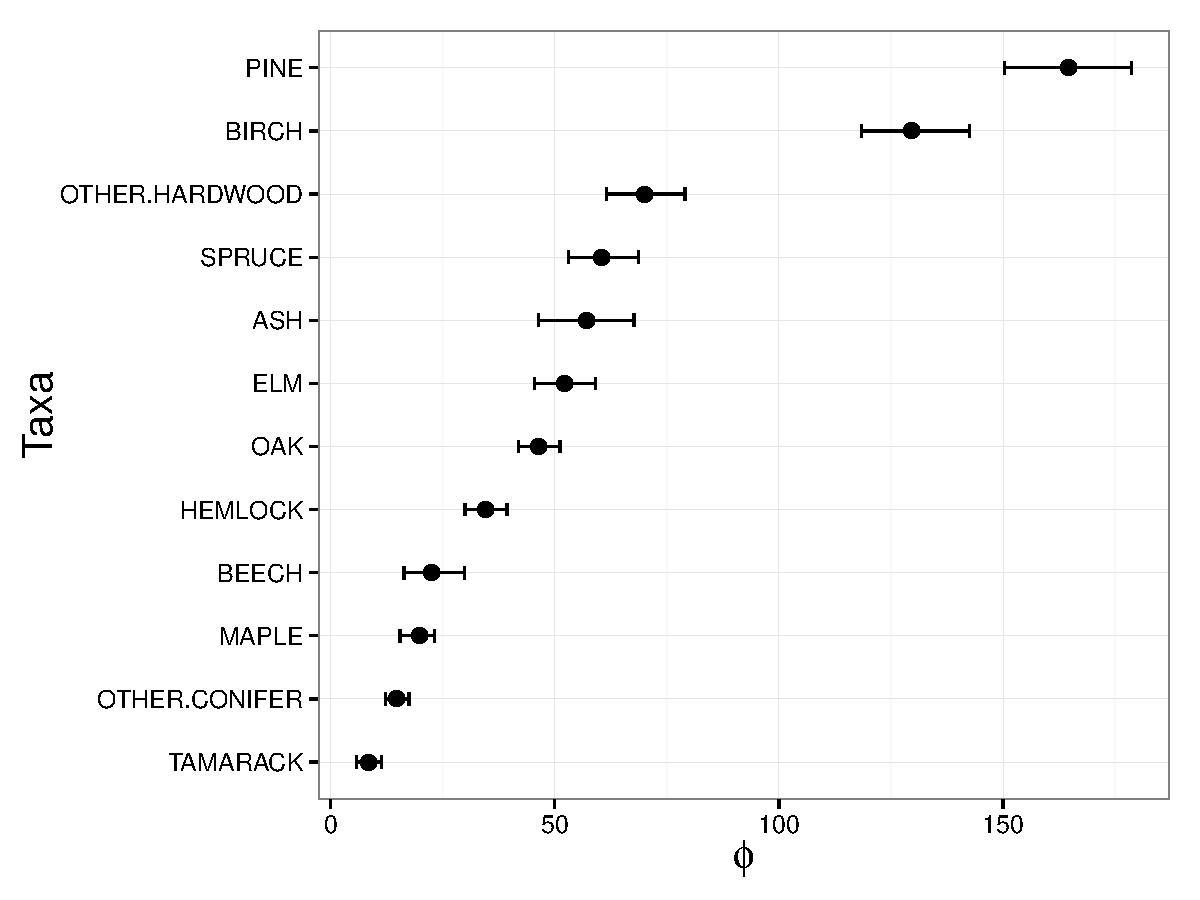
\includegraphics[width=7in]{figures/phi_vary_psi.pdf}
% \caption{Mean values of 95\% credible intervals for the estimated values of the differential production parameter $\phi$ for the case where $\psi$ varied by taxon.}
% \label{fig:phi_vary_psi}
% \end{figure}

%potential pollen maps by taxon
\begin{figure}
\centering
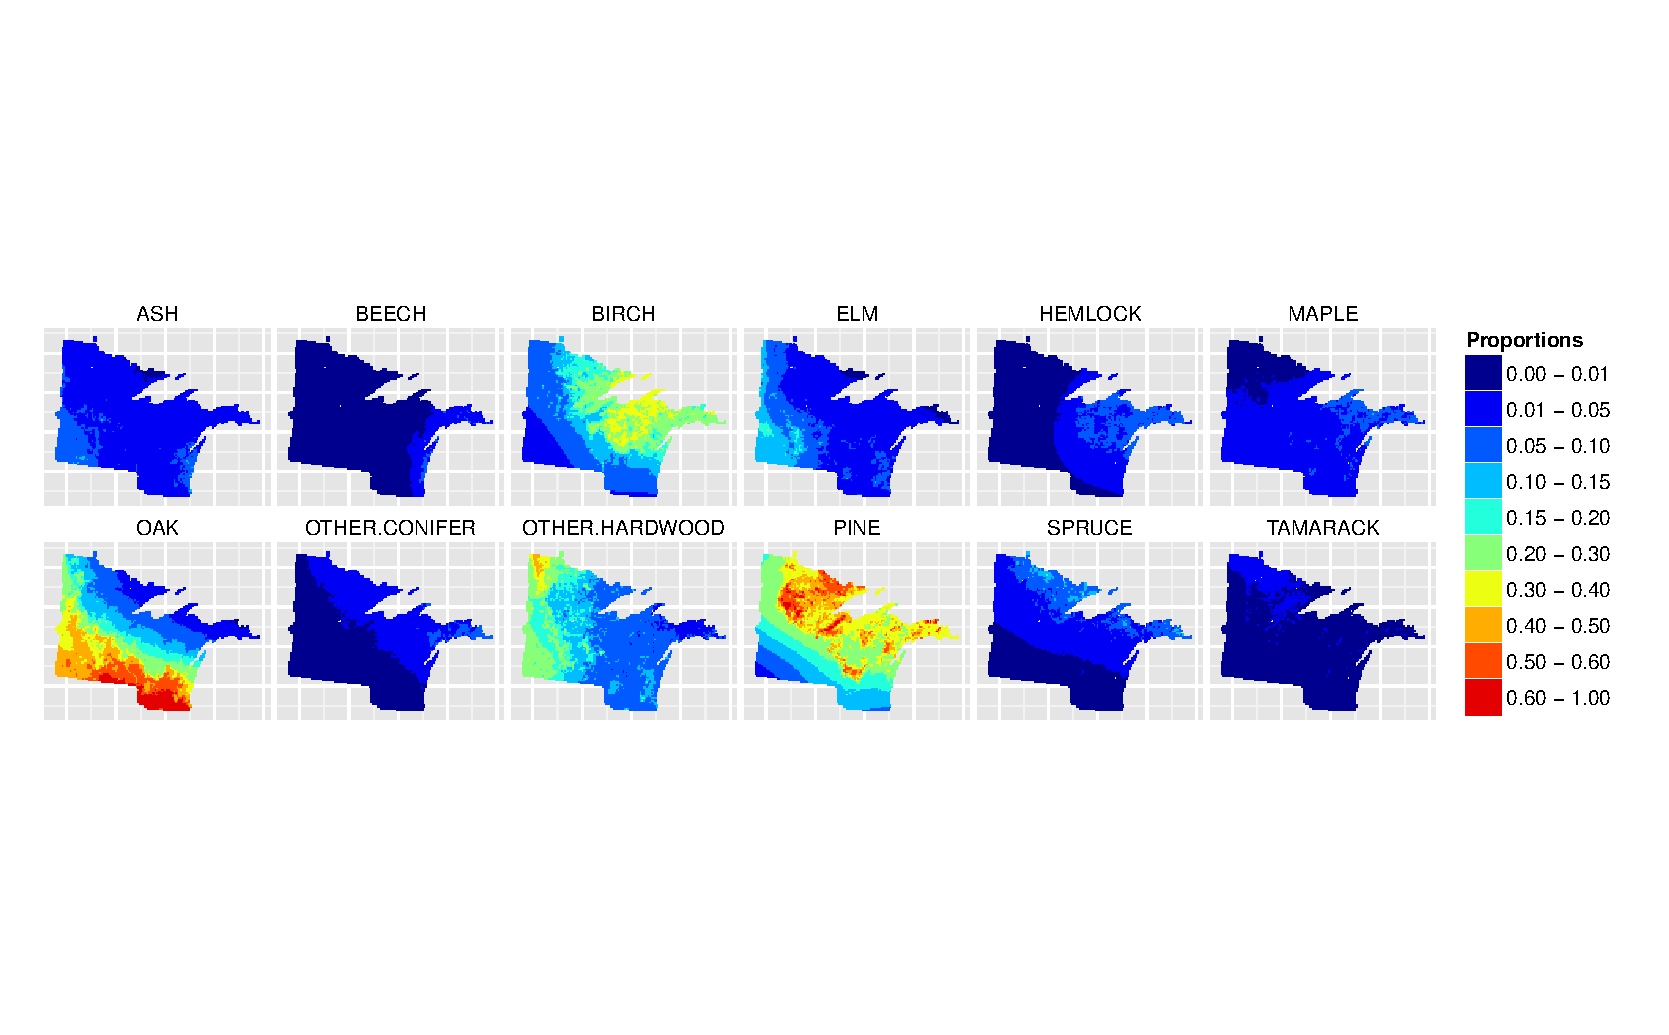
\includegraphics[width=7in]{figures/maps_pollen.pdf}
\caption{Heat maps of model-predicted pollen for each grid cell in the domain, by taxon.}
\label{fig:maps_pollen}
\end{figure}

%PLS data maps by taxon
\begin{figure}
\centering
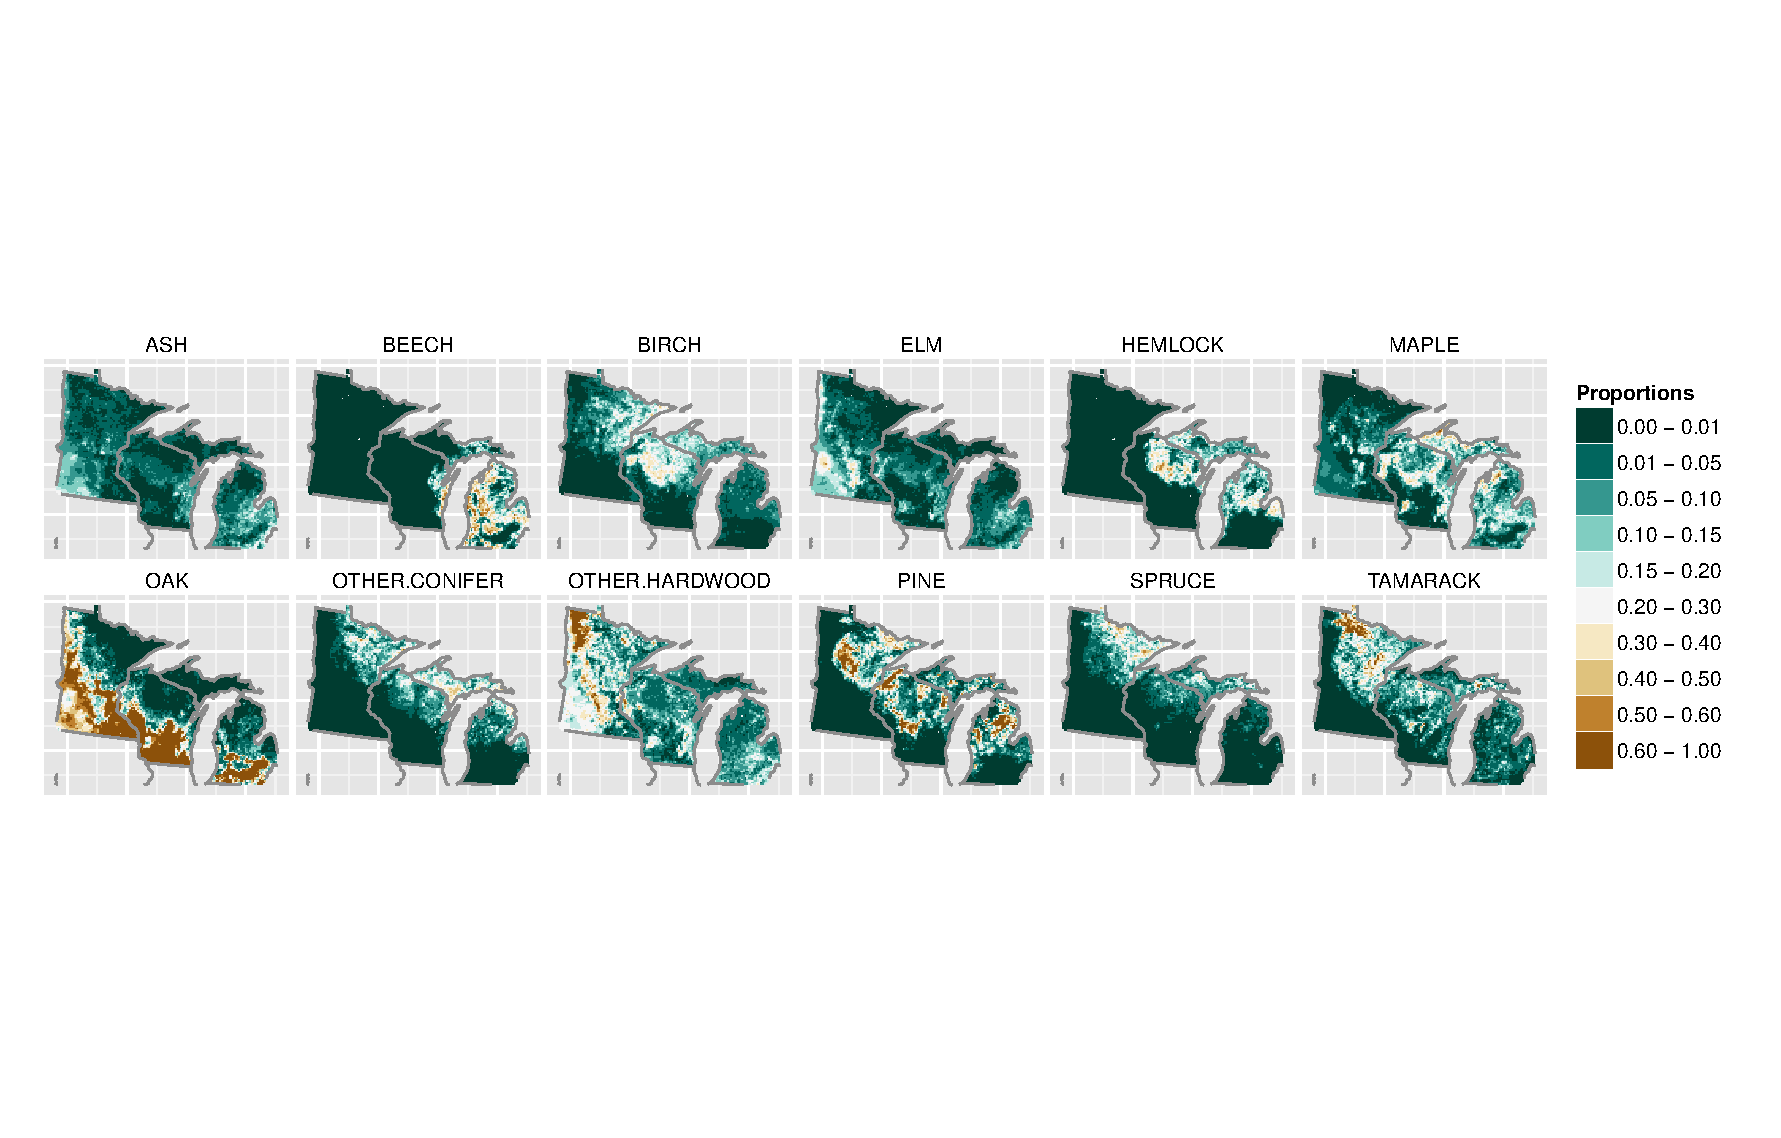
\includegraphics[width=7in]{figures/maps_veg.pdf}
\caption{Heat maps of the PLS data, by taxon.}
\label{fig:maps_veg}
\end{figure}





